\chapter{Paru-Paru dan Pertukaran Gas}\label{ch:g7:lungs-and-gas-exchange}

Setiap menit dalam hidupmu, kira-kira delapan liter udara melintasi
dua organ yang belum pernah kamu lihat. \Cref{ch:g4:breathing}
menyketsakan jalannya dan pertukarannya;
\cref{ch:g7:how-animals-breathe} menempatkan mesin manusianya di
antara keempat mesin kerajaan \omterm{def:g1:animals-around-us:animal}{hewan}. Bab ini melengkapi gambarannya:
permesinan pengudaraannya, kantong udaranya dengan nama yang
sebenarnya, bilangan pertukarannya --- dan apa yang diperbuat asap
terhadap seluruh perangkatnya.

\section{Permesinan pengudaraannya}

\begin{proposition}[Bagaimana udaranya dipindahkan]\label{prop:g7:lungs-and-gas-exchange:ventilation}
\omterm{def:g7:how-animals-breathe:four}{Paru-paru} tidak punya \omterm{def:g3:bones-and-muscles:muscle}{otot} sendiri; dadanya memompanya seperti sebuah
puputan:
\begin{itemize}
  \item \omterm{def:g4:breathing:movements}{menarik napas} adalah \emph{pekerjaan}: \omterm{def:g3:bones-and-muscles:muscle}{otot} rusuknya
        mengangkat lalu melebarkan sangkarnya, dan
        \emph{diafragma}\index{diafragma} --- lantai \omterm{def:g3:bones-and-muscles:muscle}{otot} yang lebar
        di bawah \omterm{def:g7:how-animals-breathe:four}{paru-parunya} --- mendatar ke bawah; dada yang melebar
        itu merentangkan \omterm{def:g7:how-animals-breathe:four}{paru-parunya}, dan udara mengalir masuk untuk
        mengisinya;
  \item \omterm{def:g4:breathing:movements}{mengembuskan napas}, ketika beristirahat, kebanyakan berupa
        \emph{pelepasan}: \omterm{def:g3:bones-and-muscles:muscle}{ototnya} mengendur, dada yang terentang
        melenting kembali, udaranya mengalir keluar. (Meniup lilin
        menambahkan \omterm{def:g3:bones-and-muscles:muscle}{otot} pada lentingannya.)
\end{itemize}
Kira-kira $15$ kali semenit ketika beristirahat
(\cref{def:g4:breathing:movements}), tanpa diminta
(\cref{rem:g5:brain-in-command:more}) --- dan didalamkan serta
dicepatkan sesuai permintaan
(\cref{prop:g7:organs-at-work:supply}).
\end{proposition}
\admitted

\begin{example}[Merasakan puputannya]\label{ex:g7:lungs-and-gas-exchange:feel}
Tangan di rusuk, tarik napas dalam-dalam: sangkarnya naik lalu melebar
di bawah telapakmu (\cref{ex:g4:breathing:watch}). Sekarang
terengah-engah seperti seekor anjing: embusan pendek yang cepat itu
nyaris seluruhnya \omterm{prop:g7:lungs-and-gas-exchange:ventilation}{diafragma}. Cegukan, demi kelengkapan, adalah
kedutan salah mulai milik \omterm{prop:g7:lungs-and-gas-exchange:ventilation}{diafragmanya} --- puputannya yang meletus
salah pada jadwalnya sendiri.
\end{example}

\section{Alveolus dan pertukarannya}

\begin{definition}[Alveolus]\label{def:g7:lungs-and-gas-exchange:alveoli}
Kantong udara mungil pada \cref{def:g4:breathing:organs} adalah
\emph{alveolus}\index{alveolus}: ratusan juta gelembung berdinding
tipis yang bergerombol pada ujung terhalus saluran udaranya,
masing-masing terbungkus \omterm{def:g4:heart-and-blood:vessels}{pembuluh darah} halus. Jumlah permukaannya
adalah separuh lapangan tenis pada
\cref{rem:g4:breathing:sponge} --- salinan manusia dari spesifikasi
luas-tipis-lembap pada
\cref{prop:g7:how-animals-breathe:spec}.
\end{definition}

\begin{proposition}[Pertukarannya, dalam bilangan]\label{prop:g7:lungs-and-gas-exchange:numbers}
Bandingkan udara yang masuk dengan udara yang keluar: udara yang
ditarik masuk kira-kira $21$ persen \omterm{def:g7:what-is-respiration:respiration}{oksigen} dan nyaris bebas \omterm{def:g7:what-is-respiration:respiration}{karbon
dioksida}; udara yang diembuskan turun menjadi kira-kira $16$ persen
\omterm{def:g7:what-is-respiration:respiration}{oksigen} dan naik menjadi kira-kira $4$ persen \omterm{def:g7:what-is-respiration:respiration}{karbon dioksida} (hangat
dan lembap pula ---
\cref{ex:g4:breathing:mirror}). Perbedaannya adalah pertukarannya:
menyeberangi dinding alveolusnya, \omterm{def:g7:what-is-respiration:respiration}{oksigen} menyeberang ke \omterm{prop:g4:journey-of-food:absorb}{darahnya} dan
\omterm{def:g7:what-is-respiration:respiration}{karbon dioksida} menyeberang kembali
(\cref{prop:g4:breathing:exchange}), setiap menit setiap hari.
\end{proposition}
\admitted

\begin{omfigure}
\begin{tikzpicture}
  \node[anchor=south west, inner sep=0] (img) at (0,0)
    {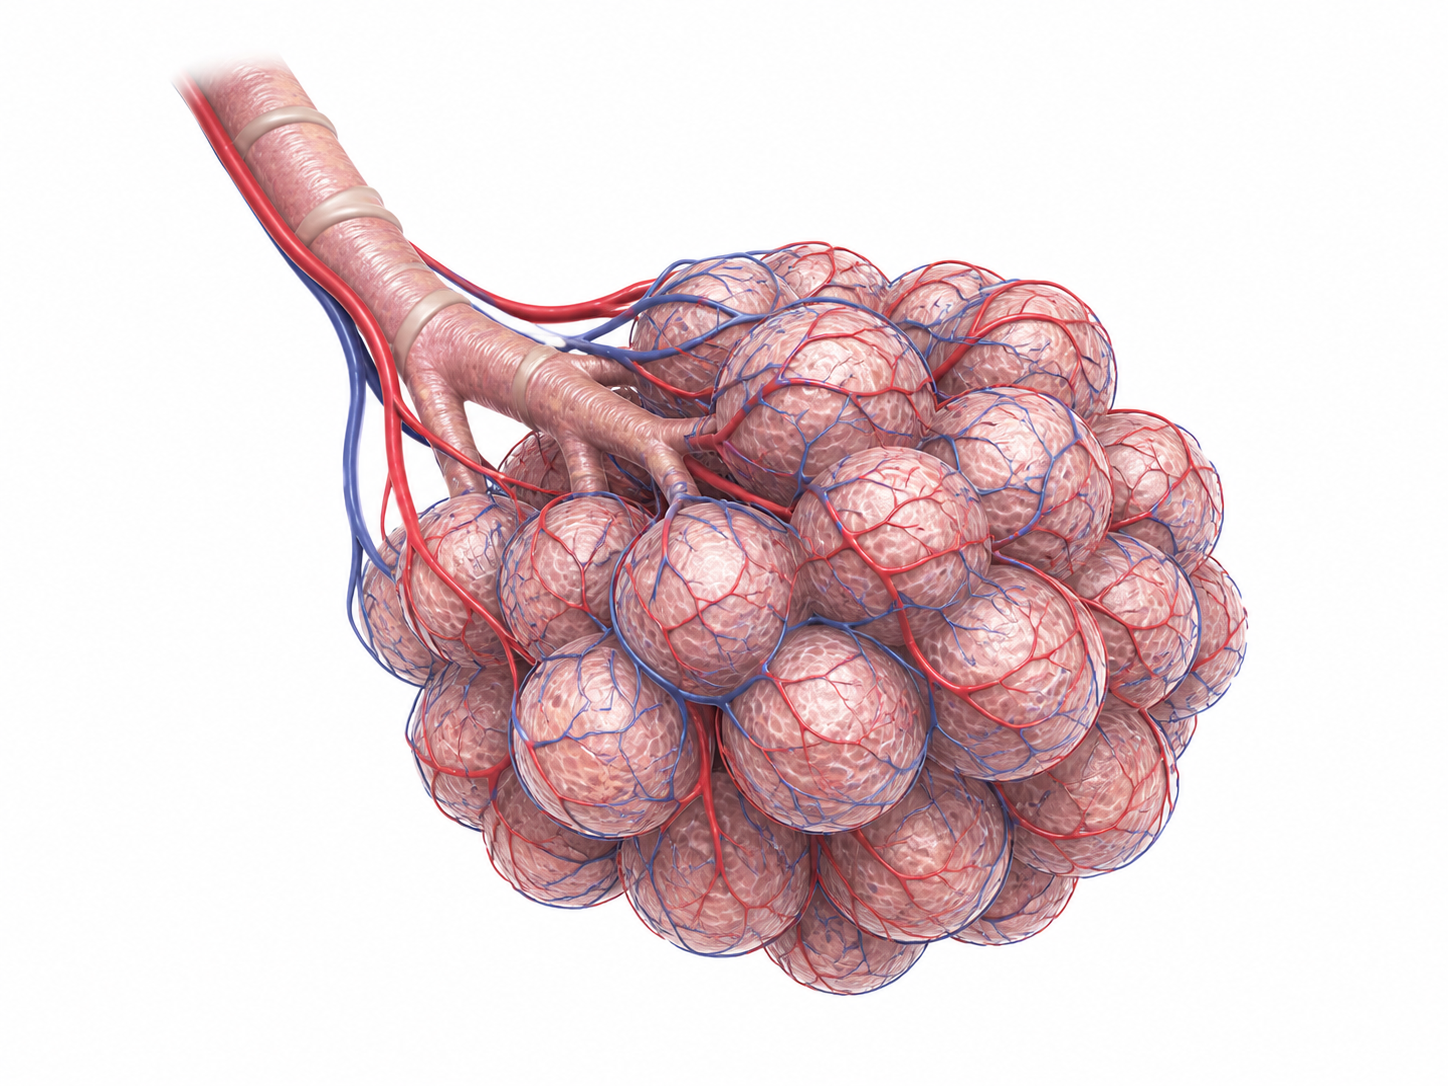
\includegraphics[width=0.6\linewidth]{images/book1/ai/fig-alveoli.png}};
  \begin{scope}[x={(img.south east)}, y={(img.north west)},
      every node/.style={font=\small}]
    \draw[omDef, thick] (0.24,0.83) -- (0.12,0.94)
      node[above] {saluran udara terhalus};
    \draw[omThm, thick] (0.78,0.62) -- (0.90,0.80)
      node[above, align=center, omThm] {pembuluh halus\\ yang membungkus};
    \draw[omMeth!60!black, thick] (0.46,0.34) -- (0.30,0.01)
      node[below, align=center, omMeth!60!black]
      {menyeberangi dinding tipis tiap gelembung:\\ oksigen ke darahnya, karbon\\
       dioksida kembali ke udaranya};
  \end{scope}
\end{tikzpicture}

{\small Satu gerombol \omterm{def:g7:lungs-and-gas-exchange:alveoli}{alveolus} di antara ratusan juta: dinding
gelembung yang tipis, bungkus \omterm{def:g4:heart-and-blood:vessels}{pembuluh} halus, dan penyeberangan dua
arah yang menjadi inti semuanya.}
\end{omfigure}

\begin{example}[Pembukuannya cocok]\label{ex:g7:lungs-and-gas-exchange:accounting}
Delapan liter semenit, seperdua puluh \omterm{def:g7:what-is-respiration:respiration}{oksigen} tiap tarikan napas yang
disimpan: hitung-hitungannya menyediakan kira-kira tagihan \omterm{def:g7:what-is-respiration:respiration}{oksigen}
tubuh yang beristirahat --- dan ketika berusaha, dengan \omterm{def:g7:what-is-respiration:respiration}{pernapasan}
yang dilipattigakan serta didalamkan dan ronde \omterm{def:g4:heart-and-blood:heart}{jantungnya} yang
dipercepat
(\cref{prop:g7:organs-at-work:supply}), pengantarannya berlipat ganda
untuk mengimbangi tagihan \omterm{def:g3:bones-and-muscles:muscle}{ototnya}. Bilangan mesinnya dan pembukuan
tubuhnya seimbang; keduanya adalah buku yang sama yang disimpan pada
dua loket.
\end{example}

\section{Permesinan yang disalahgunakan: asap}

\begin{proposition}[Apa yang diperbuat asap terhadap perangkatnya]\label{prop:g7:lungs-and-gas-exchange:smoke}
Asap tembakau menyerang setiap lantai bab ini
(\cref{prop:g5:healthy-choices:substances} sudah memberi
peringatannya; inilah keteknikannya):
\begin{itemize}
  \item tarnya melapisi dan mengiritasi saluran udaranya: permukaan
        pembersihnya melemah dan ``batuk perokok'' adalah sapu
        saluran udaranya yang kelebihan beban;
  \item dinding alveolusnya, yang teriritasi menahun, rusak:
        kantongnya bergabung menjadi ruang yang lebih sedikit, lebih
        besar dan lebih kendur --- \emph{permukaannya hilang}, dan
        bersamanya hilang pula pertukarannya (spesifikasinya, yang
        dibongkar);
  \item salah satu gas asapnya menumpangi kursi \omterm{def:g7:what-is-respiration:respiration}{oksigen} di dalam
        \omterm{prop:g4:journey-of-food:absorb}{darahnya}, sehingga mendesak \omterm{def:g7:what-is-respiration:respiration}{oksigen} turun dari
        pengangkutannya sendiri;
  \item dan saluran udaranya menyempit --- setiap tarikan napas
        melintasi dada seorang perokok adalah tarikan napas melintasi
        sebuah puputan yang sebagian tersumbat.
\end{itemize}
Kerusakannya lambat, menumpuk dan hanya sebagian dapat dipulihkan:
\omterm{def:g7:how-animals-breathe:four}{paru-paru} yang tidak pernah memulai mempertahankan separuh lapangan
tenisnya secara utuh (\cref{rem:g5:healthy-choices:never}).
\end{proposition}
\admitted

\begin{example}[Dua uji tangga]\label{ex:g7:lungs-and-gas-exchange:stairs}
Ketiga lantai pada \cref{ch:g7:organs-at-work}, yang didaki dua orang
dewasa yang setara umur dan kebiasaan latihannya, satu di antaranya
seorang perokok jangka panjang: si perokok tiba terengah-engah pada
\omterm{prop:g4:heart-and-blood:pulse}{denyut nadi} yang baru dicapai yang lain ketika berlari cepat.
Permukaan yang lebih sedikit, kursi yang terisi, saluran udara yang
menyempit --- rantai pasokannya membayar tagihan
\cref{prop:g7:organs-at-work:bill} lewat sebuah pemasukan yang
tercekik. Uji kebugaran membaca sejarah \omterm{def:g7:how-animals-breathe:four}{paru-parunya} sepasti pemindaian
mana pun.
\end{example}

\begin{method}[Menjaga permesinannya]\label{met:g7:lungs-and-gas-exchange:keep}
\Cref{met:g4:breathing:care}, yang ditingkatkan dengan alasan bab ini:
\begin{enumerate}
  \item jangan ada asap --- asapmu atau asap orang lain: permukaan
        yang hilang nyaris tidak diperoleh kembali;
  \item anginkan ruangannya (\cref{exo:g4:breathing:10}) dan pilihlah
        udara luar yang bersih untuk berolahraga;
  \item latihlah puputannya: usaha yang menuntut napas dalam membangun
        \omterm{def:g3:bones-and-muscles:muscle}{otot} \omterm{def:g7:what-is-respiration:respiration}{pernapasannya} dan menjaga seluruh permukaannya tetap
        terudarai;
  \item bernapaslah lewat hidung di udara dingin dan berdebu
        (\cref{exo:g4:breathing:7}) --- penyaringnya melindungi
        sapunya.
\end{enumerate}
\end{method}

\section{Latihan}

\begin{exercise}[$\star$]\label{exo:g7:lungs-and-gas-exchange:1}
Lukiskan \omterm{def:g4:breathing:movements}{menarik napas} dan \omterm{def:g4:breathing:movements}{mengembuskan napas} sebagai pekerjaan dan
pelepasan: \omterm{def:g3:bones-and-muscles:muscle}{otot} yang mana, gerakan yang mana?
\end{exercise}

\begin{exercise}[$\star$]\label{exo:g7:lungs-and-gas-exchange:2}
Apa itu \omterm{prop:g7:lungs-and-gas-exchange:ventilation}{diafragma}, dan di mana ia bertempat?
\end{exercise}

\begin{exercise}[$\star$]\label{exo:g7:lungs-and-gas-exchange:3}
Apa itu \omterm{def:g7:lungs-and-gas-exchange:alveoli}{alveolus} --- berapa banyak, berdinding bagaimana, terbungkus
apa?
\end{exercise}

\begin{exercise}[$\star$]\label{exo:g7:lungs-and-gas-exchange:4}
Berikan bilangan bulatnya: \omterm{def:g7:what-is-respiration:respiration}{oksigen} di udara yang ditarik masuk, di
udara yang diembuskan; \omterm{def:g7:what-is-respiration:respiration}{karbon dioksida} di udara yang diembuskan. Berapa
perbedaannya?
\end{exercise}

\begin{exercise}[$\star$]\label{exo:g7:lungs-and-gas-exchange:5}
Spesifikasi mana yang dipenuhi alveolusnya, dan dengan dua organ lain
pada tahun ini yang mana ia membaginya?
\end{exercise}

\begin{exercise}[$\star$]\label{exo:g7:lungs-and-gas-exchange:6}
Sebutkan tiga di antara keempat serangan asap terhadap permesinannya.
\end{exercise}

\begin{exercise}[$\star\star$]\label{exo:g7:lungs-and-gas-exchange:7}
Mengapa \omterm{def:g4:breathing:movements}{menarik napas} itu pekerjaan sedangkan \omterm{def:g4:breathing:movements}{mengembuskan napas}
ketika beristirahat itu gratis? Dari mana datangnya dorongan ke luar?
\end{exercise}

\begin{exercise}[$\star\star$]\label{exo:g7:lungs-and-gas-exchange:8}
Jelaskan mengapa permukaan \omterm{def:g7:lungs-and-gas-exchange:alveoli}{alveolus} yang hilang tidak dapat
diimbangi dengan bernapas lebih cepat --- faktor pertukaran mana yang
hilang?
\end{exercise}

\begin{exercise}[$\star\star$]\label{exo:g7:lungs-and-gas-exchange:9}
Tafsirkan kedua uji tangga pada
\cref{ex:g7:lungs-and-gas-exchange:stairs} serangan demi serangan.
\end{exercise}

\begin{exercise}[$\star\star$]\label{exo:g7:lungs-and-gas-exchange:10}
Seorang penyelam \omterm{def:g4:breathing:movements}{mengembuskan napas} pelan-pelan ketika naik ke
permukaan; seorang pemain terompet menahan nada panjang yang mantap.
Paruh yang mana dari
\cref{prop:g7:lungs-and-gas-exchange:ventilation} yang masing-masing
mereka latih atau pakai?
\end{exercise}

\begin{exercise}[$\star\star$]\label{exo:g7:lungs-and-gas-exchange:11}
Damaikan \cref{ex:g7:lungs-and-gas-exchange:accounting} dengan
\cref{prop:g7:organs-at-work:supply}: tiga penyetelan mana yang
melipatgandakan pengantaran ketika berusaha, dan pada loket yang mana?
\end{exercise}

\begin{exercise}[$\star\star\star$]\label{exo:g7:lungs-and-gas-exchange:12}
``\omterm{def:g7:how-animals-breathe:four}{Paru-paru} adalah sebuah perbatasan seluas separuh lapangan tenis
yang terlipat di dalam sebuah kotak sepatu, dan asap adalah api yang
lambat di perbatasan itu.'' Belalah kedua gambaran itu dengan bilangan
dan mekanisme bab ini.
\end{exercise}

\section{Soal: Berkas Mesin Pernapasan}

\begin{problem}[{Soal akhir pekan --- pemeriksaan seorang insinyur
atas puputan manusia}]\label{pb:g7:lungs-and-gas-exchange:1}
Sebuah kelas keteknikan ``memeriksa'' mesin \omterm{def:g7:what-is-respiration:respiration}{pernapasan} manusia di atas
kertas: pemasukan, pompa, permukaan pertukaran, sambungan
pengangkutan, dan catatan pemeliharaan.

\medskip\noindent\textbf{Bagian I --- Pompanya.}
\begin{enumerate}
  \item Susunlah daur pompanya: kedua tahapnya, penggerak
        masing-masingnya, dan tahap mana yang berharga \omterm{prop:g3:balanced-diet:jobs}{energi} ketika
        beristirahat.
  \item Pompanya tidak bersentuhan dengan \omterm{def:g3:bones-and-muscles:muscle}{otot} organ yang dipompanya
        --- \omterm{def:g7:how-animals-breathe:four}{paru-parunya} tidak punya \omterm{def:g3:bones-and-muscles:muscle}{otot}. Bagaimana pelebaran dadanya
        sama sekali dapat memindahkan udara?
  \item Berikan laju istirahat pompanya dan kedua penyetelan usahanya
        (\cref{prop:g7:organs-at-work:supply}).
  \item Terengah-engah, mendesah, meniup lilin: berikan kepada
        masing-masingnya tempatnya di dalam mekanika daurnya.
\end{enumerate}

\medskip\noindent\textbf{Bagian II --- Permukaan
pertukarannya.}
\begin{enumerate}[resume]
  \item Rincikan permukaannya: nama, jumlah, dinding, bungkus, ukuran
        seluruhnya.
  \item Periksalah spesifikasinya terhadap
        \cref{prop:g7:how-animals-breathe:spec}, butir demi butir.
  \item Udara pemasukan dan udara buangannya berbeda menurut persentase
        bab ini. Hitunglah perbedaan \omterm{def:g7:what-is-respiration:respiration}{oksigennya} sebagai pecahan dari
        $21$ persen pemasukannya --- kasarnya berapa bagian \omterm{def:g7:what-is-respiration:respiration}{oksigen}
        yang ditarik masuk yang disimpan?
  \item Mengapa udara buangannya harus tetap hangat dan lembap ---
        sifat permukaan yang mana yang menjadikannya harga bayarannya?
\end{enumerate}

\medskip\noindent\textbf{Bagian III --- Catatan
pemeliharaannya.}
\begin{enumerate}[resume]
  \item Arsipkan keempat serangan asapnya di bawah: pemasukan, pompa,
        permukaan, pengangkutan. Satu baris masing-masing.
  \item Berkasnya mencatat: ``kehilangan permukaan adalah kehilangan
        modal.'' Jelaskan, dibandingkan dengan batuk dan pilek yang
        merupakan perbaikan berjalan.
  \item Tuliskan jadwal pemeliharaannya ---
        \cref{met:g7:lungs-and-gas-exchange:keep} --- sebagai empat
        arahan insinyur beserta alasannya.
  \item Simpulkan pemeriksaannya: satu kalimat tentang mengapa mesin
        ini, satu-satunya di antara pompa dan perbatasan tubuhnya,
        setengahnya berada di bawah kendali sukarela pemiliknya ---
        dan untuk apa kendali itu (berbicara, bernyanyi, embusan pelan
        sang penyelam).
\end{enumerate}
\end{problem}
